% This is the Reed College LaTeX thesis template. Most of the work
% template. Later comments etc. by Ben Salzberg (BTS). Additional
% restructuring and APA support by Jess Youngberg (JY).
% Your comments and suggestions are more than welcome; please email
% them to cus@reed.edu
%
% See http://web.reed.edu/cis/help/latex.html for help. There are a
% great bunch of help pages there, with notes on
% getting started, bibtex, etc. Go there and read it if you're not
% already familiar with LaTeX.
%
% Any line that starts with a percent symbol is a comment.
% They won't show up in the document, and are useful for notes
% to yourself and explaining commands.
% Commenting also removes a line from the document;
% very handy for troubleshooting problems. -BTS

% As far as I know, this follows the requirements laid out in
% the 2002-2003 Senior Handbook. Ask a librarian to check the
% document before binding. -SN

%%
%% Preamble
%%
% \documentclass{<something>} must begin each LaTeX document
\documentclass[12pt,twoside]{reedthesis}
% Packages are extensions to the basic LaTeX functions. Whatever you
% want to typeset, there is probably a package out there for it.
% Chemistry (chemtex), screenplays, you name it.
% Check out CTAN to see: http://www.ctan.org/
%%
\usepackage{graphicx,latexsym}
\usepackage{amsmath}
\usepackage{amssymb,amsthm}
\usepackage{longtable,booktabs,setspace}
\usepackage{chemarr} %% Useful for one reaction arrow, useless if you're not a chem major
\usepackage{rotating}

% Modified by CII
\usepackage[hyphens]{url}
\usepackage{hyperref}
\usepackage{lmodern}

% Added by CII (Thanks, Hadley!)
% Use ref for internal links
\renewcommand{\hyperref}[2][???]{\autoref{#1}}
\def\chapterautorefname{Chapter}
\def\sectionautorefname{Section}
\def\subsectionautorefname{Subsection}

\usepackage{caption}
\captionsetup{width=5in}

% \usepackage{times} % other fonts are available like times, bookman, charter, palatino

\title{Political Ideology and Congressional Leadership}
\author{John R. Trautlein, Jr.}
% The month and year that you submit your FINAL draft TO THE LIBRARY (May or December)
\date{May 2016}
\division{History and Social Sciences}
\advisor{Alexander H. Montgomery}
%If you have two advisors for some reason, you can use the following
%%% Remember to use the correct department!
\department{Political Science}
% if you're writing a thesis in an interdisciplinary major,
% uncomment the line below and change the text as appropriate.
% check the Senior Handbook if unsure.
%\thedivisionof{The Established Interdisciplinary Committee for}
% if you want the approval page to say "Approved for the Committee",
% uncomment the next line
%\approvedforthe{Committee}

% Below added by CII

%%% Copied from knitr
%% maxwidth is the original width if it's less than linewidth
%% otherwise use linewidth (to make sure the graphics do not exceed the margin)
\makeatletter
\def\maxwidth{ %
  \ifdim\Gin@nat@width>\linewidth
    \linewidth
  \else
    \Gin@nat@width
  \fi
}
\makeatother

\renewcommand{\contentsname}{Table of Contents}

\setlength{\parskip}{0pt}


\providecommand{\tightlist}{%
  \setlength{\itemsep}{0pt}\setlength{\parskip}{0pt}}

\Acknowledgements{
Will add acknowledgements after orals.
}

\Dedication{
Will add dedication after orals.
}

\Preface{

}

\Abstract{
This paper examines the differences in ideology in Congress between
non-leaders and congressional leaders, the speakers, and whips. While
past research has looked at the ideology of congressional leaders before
they have taken their positions of power they have neglected to look at
how their ideology changes as they have taken to their new position
within the congressional power structure. Using measures of ideology
from a \texttt{NOMINATE} dataset we fit models based on party and
leadership status. The leaders are then compared to the non-leaders on
how their ideology changes compared to the mean ideology of Congress at
the time and the models are assessed for statistical significance.
Results are then expanded on and a discussion follows.
}

\usepackage{setspace}

%%
%% End Preamble
%%
%

\begin{document}

      \maketitle
  
  \frontmatter % this stuff will be roman-numbered
  \pagestyle{empty} % this removes page numbers from the frontmatter

      \begin{acknowledgements}
      Will add acknowledgements after orals.
    \end{acknowledgements}
  
  
  % Add table of abbreviations?

      \hypersetup{linkcolor=black}
    \setcounter{tocdepth}{2}
    \tableofcontents
  
      \listoftables
  
      \listoffigures
  
      \begin{abstract}
      This paper examines the differences in ideology in Congress between
      non-leaders and congressional leaders, the speakers, and whips. While
      past research has looked at the ideology of congressional leaders before
      they have taken their positions of power they have neglected to look at
      how their ideology changes as they have taken to their new position
      within the congressional power structure. Using measures of ideology
      from a \texttt{NOMINATE} dataset we fit models based on party and
      leadership status. The leaders are then compared to the non-leaders on
      how their ideology changes compared to the mean ideology of Congress at
      the time and the models are assessed for statistical significance.
      Results are then expanded on and a discussion follows.
    \end{abstract}
  
      \begin{dedication}
      Will add dedication after orals.
    \end{dedication}
  
  \mainmatter % here the regular arabic numbering starts
  \pagestyle{fancyplain} % turns page numbering back on

  \doublespacing
  
  \chapter*{Introduction}\label{introduction}
  \addcontentsline{toc}{chapter}{Introduction}
  
  This paper examines the differences in ideology in Congress between
  non-leaders and congressional leaders, the speakers, and whips. While
  past research has looked at the ideology of congressional leaders before
  they have taken their positions of power they have neglected to look at
  how their ideology changes as they have taken to their new position
  within the congressional power structure. Using measures of ideology
  from a \texttt{NOMINATE} dataset we fit models based on party and
  leadership status. The leaders are then compared to the non-leaders on
  how their ideology changes compared to the mean ideology of Congress at
  the time and the models are assessed for statistical significance.
  
  \chapter{Literature Review}\label{literature-review}
  
  \section{Congressional Leaders}\label{congressional-leaders}
  
  Party leaders are hugely important in Congress. Perhaps their most
  important role is setting the legislative agenda in Congress (Rohde
  1991, @Sinclair1983). By setting the agenda in arguably the most
  powerful branch of government, congressional leaders have extraordinary
  power over which bills are brought to a vote and eventually passed. They
  also have the power of being able to shift congressional actions away
  from an otherwise sipmles answer to a problem.\footnote{For a recent
    example of this, see how in 2008 Harry Reid (D) then the majority
    leader of the Senate, was able to remove the possibility of a nuclear
    waste repository from being created at Yucca Mountain.} Leaders in
  Congress have large sway over the leaders who they can choose to fill
  the many roles below them. They are also the ``brand image'' of their
  party, especially when their party does not control the presidency.
  Understanding the ideology of leaders is important for a Congressional
  scholar to better understand why leaders act the way the do.
  
  There has often been the question of whether or not congressional
  leaders are moderates in their party, near to their party's mean, or
  extremists. Moderates would often be effective legislators, as they
  would be able to propose more centrist policies that might apply to both
  political parties. Extremists might be selected due to their ability to
  placate the louder wings of both the Republican and Democratic parties.
  A political scientist or an economist might be quick to answer that a
  congressperson near the median voter in a political party has a strong
  theoretical reasoning for being chosen.
  
  Understanding what a median voter is as well as the median voter theorem
  is important for many quantitative approaches to the study of political
  ideology. A median voter is the voter in the middle of a group of voters
  measured among one or more
  dimensions.\footnote{As the number of dimensions increases however it can get more complicated to decide which voter is in fact the median voter. You have to properly scale each dimension to make sure some do not overpower others.}
  An table of voters is displayed below with their names and respective
  ideologies, picked from the actual numbers from the Nokken and Poole
  version of the D-NOMINATE dataset. These are the first dimensions
  scores, often categorized as ideology, with -1 being extreme liberalism
  and 1 being extreme conservatism. They are from the 113th Congress, the
  most recent Congressional session available in the dataset.
  
  \begin{table}[]
  \centering
  \caption{Ideologies Presented for Median Voter Theorem Example}
  \begin{tabular}{l|r}
  Name      & Ideology \\ \hline
  Warren    & -0.538   \\
  Reid      & -0.422   \\
  Wyden     & -0.381   \\
  Warner    & -0.238   \\
  Collins   & 0.061    \\
  McCain    & 0.367    \\
  Rubio     & 0.531    \\
  McConnell & 0.568    \\
  Cruz      & 0.754   
  \end{tabular}
  \end{table}
  
  Here the median voter would be Senator Susan Collins, as her ideology,
  0.061, puts her at the middle point, or the median, of the list of
  voters. The median voter theorem applies in majoritarian voting systems.
  The median voter, in this circumstance Senator Collins, will have their
  preferred outcome chosen by the voters in the system. A majoritarian
  voting system is when a vote is won when more than half of the votes are
  for a specific option. This is different than a plurality system, which
  just makes whichever has the most votes the winner, regardless of
  whether or not they have a majority of the votes. For example, if 40\%
  voted for option A, 30\% voted for option B, and 30\% voted for option C
  then options A would be chosen under plurality rule, but not under
  majority rule. One of the options would need to be more than 50\%. If
  say in a new vote option D got 50\% of the vote that would not be enough
  to win in a majoritarian system as option E could also have 50\% of the
  vote at the same time.
  
  To continue the discussion above, the reason why you might expect the
  congressperson elected to serve a leadership position to occupy the
  median space in the party is because in these elections the votes taken
  solely within the party.\footnote{With the exception of the vote for
    Speaker in the House of Representatives, although that vote often ends
    up being made up entirely of the majority party's congresspersons
    voting in affirmation with the minority party avoiding casting a
    positive ballot.} The median voter theorem states that ``a majority
  rule voting system will select the outcome most preferred by the median
  voter'' (Holcombe 2006, 115). This builds off the assumption that there
  is only one dimension along which politics exists, for example, left to
  right or liberal to conservative. Is it also assumed that a voter will
  choose the option, or in this circumstance the politician, closest to
  their own ideal point along the singular dimension. In a majoritarian
  system this ideal median point will prevail, having more than 50\% of
  the vote in the final vote tallied.
  
  Studies have examined where leaders come from ideologically speaking.
  One has found, using the DW-NOMINATE scores of congressional leaders,
  that these leaders do in fact come from near the median of their party,
  with a tiny preference towards the slightly more extreme candidate,
  left-leaning for Democrats and right-leaning for Republicans.
  DW-NOMINATE scores place congresspersons on a single dimension from -1
  to 1, with -1 being left-leaning and 1 being right-leaning. The numbers
  are found by taking the roll call votes over a single Congress and then
  placing the legislator's scores within the range of possible values. A
  senator like Ted Cruz would end up with a number close to 1\footnote{In
    the 113th Congress his point was measured at 0.754.} whereas for
  senator like Elizabeth Warren you would see a point near to -1\footnote{In
    the 113th Congress her point was measured at -0.538}. House Democrats
  were found to be on average -0.050 away from the median point whereas
  their leaders were on overage -0.097, slightly farther away but still
  close to the median. For Senate Democrats these numbers are 0.016 and
  -0.059 respectively, again the the leaders being slighly more extreme
  than the median but still being quite close to it. For the Republicans
  the results are similar, although in the other direction. In the House,
  for leaders the average distance away from the party median for leaders
  is 0.044 whereas for the rest of the House Republicans it is -0.025. For
  the Senate Republicans the numbers are 0.048 and 0.057,
  respectively.\footnote{The Republicans in the Senate are the only group
    who elect leaders slightly more moderate on average than the party
    median in that chamber.} They find it ``hearening to note that
  leaders--who some political observers argue have strong influence over
  angenda setting and lawmaking under certain conditions--are, on balance,
  fairly representative of their parties. If leaders came from the far
  extremes of the chambers\ldots{}then policy might be even less
  reflective of the preferences of the median voter in the electorate''
  (Jessee and Malhotra 2010, see specifically 386). Jessee and Malhotra
  (2010) also find that the winner of a congressional leadership race is
  not ``ideologically distinctive'' from the entire pool candidates (2010,
  361).
  
  This evidence found in Jessee and Malhotra (2010) looked to revise
  earlier studies on the subject. Harris and Nelson (2008) looked at the
  old ``Austin-Boston'' alliance that encourage the selection of middlemen
  in the Democratic party, and also examine the changes within the
  Republican party leadership as well. Surprised by the election of the
  relatively extreme Pelosi to the Speakership, the two authors felt the
  need to revisit the question of whether the median voter theorem still
  held.\footnote{While the middle\emph{men} theory could still hold, the
    middle\emph{person} theory was in doubt.} Using the same dataset as
  Jessee and Malhotra (2010), they came to a new conclusion, that perhaps
  more partisan leaders were need as political polarization increased.
  Seeing the role switch from a place for compromise during a ``bargaining
  era and bipartisan Congress'' to a new bully pulpit, often active in the
  media and courting donors, middlepersons seemed to no longer be the most
  appropriate leaders of their party on the national stage of Congress
  (Harris and Nelson 2008, 54). Their final hypothesis is that as partisan
  divisions increase it will exacerbate the extremism of congressional
  leaders.
  
  Older research is more theoretical and is less likely to use datasets,
  like the many NOMINATE datasets available. In May (1973) leaders are
  suggested to be more extreme than the rest of their party when ideology
  is strongly important, which may connect well to the modern era. Studies
  of both British and Norwegian legislative systems cast doubt on May's
  concept, the law of curvilinear disparity.\footnote{,,todo - Unlikely
    that I should go into more depth, but maybe I could within a footnote?}
  The middleman theory is further promoted by Clausen and Wilcox (1987),
  who finds the best support for the theory in the House and then best
  within the Democratic party, which had at the time been the majority
  power for 32 years. Quickly stated, they claim that ``leaders are chosen
  who are\ldots{}dedicated to represent and prosecute the party position''
  (Clausen and Wilcox 1987, 261). More studies find evidence that leaders
  are more extreme than the median voter theorem would suggest, as
  Grofman, Koetzle, and McGann find that Democratic leaders are to the
  left of the median of their party and Republican leaders are to the
  right of the median of their party (Grofman, Koetzle, and McGann
  (2002)).
  
  \section{DW-NOMINATE}\label{dw-nominate}
  
  Keith Poole's and Howard Rosenthal's previous work about congressional
  ideology is the backbone of this study. they have constructed a way to
  fit members of Congress across a unidimensional metric that measures
  primarily ideology. Their typical dataset measures a single ``ideal
  point'' for each congressperson throughout their career and is able to
  plot them against other members of Congress throughout its existence.
  There are alternative versions of their dataset that also exist, and I
  use the Nokken and Poole version, which allows members to shift their
  ideology throughout different sessions of Congress (Nokken and Poole
  2004). There is often a clamoring by many for the structure of Congress
  to be displayed in multiple different dimesions, sometimes even one
  dimension for every issue available. More often however there is a
  request for a second dimension that allows not just a conservative
  versus liberal axis but instead a socially liberal versus socially
  conservative axis and a fiscally liberal versus fiscally conservative
  axis. While at times a second axis is useful, and in the most recent
  session of Congress can be viewed as a measure of establishment versus
  non-establishment leanings, Poole and Rosenthal as well as those who
  have use their datasets in the past primarily look to create their
  models solely from this one dimension due to its explanatory power
  (Poole and Rosenthal 2007, 21). Part of the reason why complicated
  legislators are able to represented along a single metric is due to the
  prevalence of logrolling or vote trading (Poole and Rosenthal 2007, 17).
  The primary dimension is not solely concerned with political party
  however, it also strongly relates to issues of economic redistribution
  (Poole and Rosenthal 2007, 70).
  
  Looking ahead to how the legislators, specifically the leaders, might
  change within my own study is evidence that ``essentially all movement
  is captured by simple linear movement'' along the single explanatory
  dimension, which suggests that more complicated ideological flip flops
  are rare within Congress (Poole and Rosenthal 2007, 29).\footnote{,,todo-would
    love to include more on this at some point}
  
  Poole and Rosenthal are able to look at the patterns of how ideology has
  changed in the history of Congress. I will solely be looking at post-WW2
  data as that is when congressional leadership started becoming truly
  strong in both the House and Senate.\footnote{Before that it was
    sometimes non-existant, especially in the smaller Senate, where
    leadership was not needed as much to organize the many members of each
    party.} They note that ``{[}t{]}he period from the late New Deal until
  the mid-1970s saw the development of the only genuine
  three-political-party system in American history. The southern and
  northern Democrats may have joined together to organize the House and
  Senate but they were widely separated on the second dimension. This
  dimension picked up conflict over civil rights'' (Poole and Rosenthal
  2007, 54). During this time there was a conservative coalition between
  the southern Democrats and most Republicans that was in conflict with
  the northern Democrats as well a a few northern Republicans (Poole and
  Rosenthal 2007, 54--56). It is unfortunate that this sole time of a
  three-political-party sytem exists during the data that I plan to use,
  but this may make my results stronger in less turbulant times. By the
  ``mid-to-late 1970s the party-line voting returned to a more
  {[}unidimensional{]} pattern'' (Poole and Rosenthal 2007, 57). This was
  due to the passage of civil rights legislation that either revolved
  conflicts within the parties or caused legislators to switch from one
  party to another Throughout the rest of congressional history the single
  dimension remains but what the dimensions refers to evolves slowly.
  Within each individual Congress it is easy to see the majority of
  conflicts along a single dimension (MacDonald and Rabinowitz 1987).
  
  Something that should help my analysis is the movement towards a more
  ``unidimesional politics'' in the most recent sessions of Congress. The
  ideological overlap along this single dimension between the parties is
  essentially gone. The last Congress in which there was an overlap in the
  Senate was the 109th, which ended in early 2007. The second dimension
  has lost much of it's explanatory power towards party since the 104th
  Congress, which began in 1995. Poole and Rosenthal say that ``the modern
  Congress is turly unidimensional'' in 2005, which was before the even
  greater polarization that began then and continues to move the two
  parties father apart (Poole and Rosenthal 2007, 55). The first
  dimension, while often refered to as ``ideology,'' can be though of in a
  few different ways. It could be that the dimension is ``thought of as
  ranging from strong loyalty to one party'' to a strong dislike of the
  policies of another party; this can often explain the placement of many
  independent or otherwise third-party congressmen\footnote{As every
    third-party Representative or Senator has been a man.} existing
  seemingly deep within another party (Poole and Rosenthal 2007, 55).
  
  Poole and Rosenthal put dimensionality and roll call voting agendas well
  in the following quote: ``In a nutshell, the roll cal voting agenda of
  Congress is always a cornucopia of diverse issues, even if many issues
  are screened from the agenda. This diversity notwithstanding, to the
  extent that spatial models are useful in describing the roll call voting
  data, only low-dimensional models are needed'' (2007, 69).
  
  \begin{center}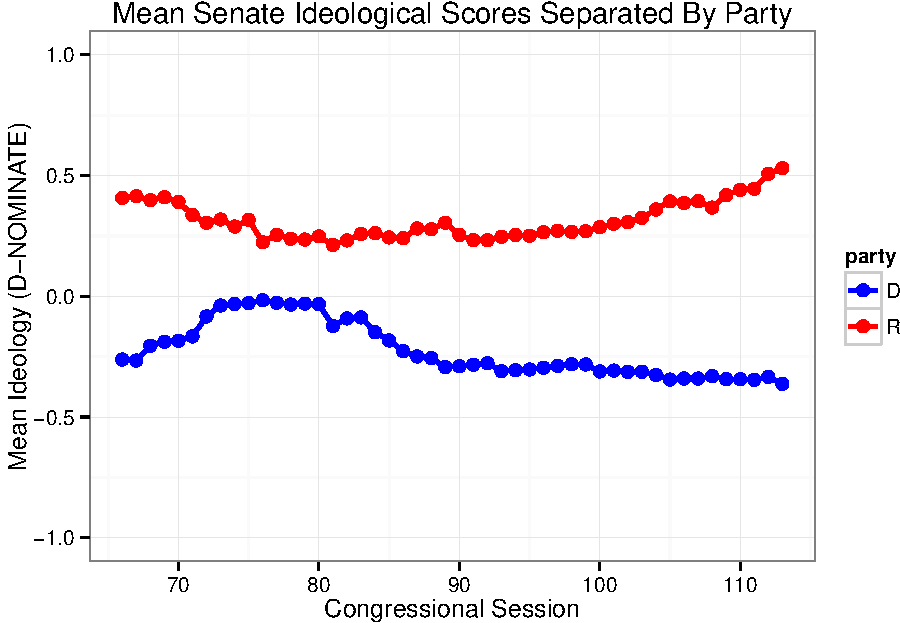
\includegraphics{trautlein_thesis_files/figure-latex/plotted_senate_means-1} \end{center}
  
  \begin{center}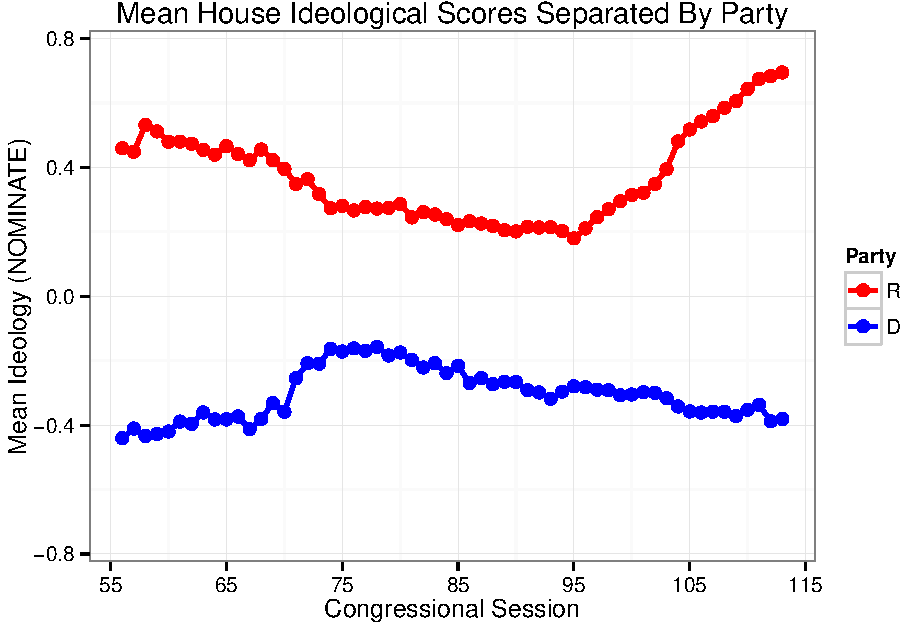
\includegraphics{trautlein_thesis_files/figure-latex/plotted_house_means-1} \end{center}
  
  \begin{center}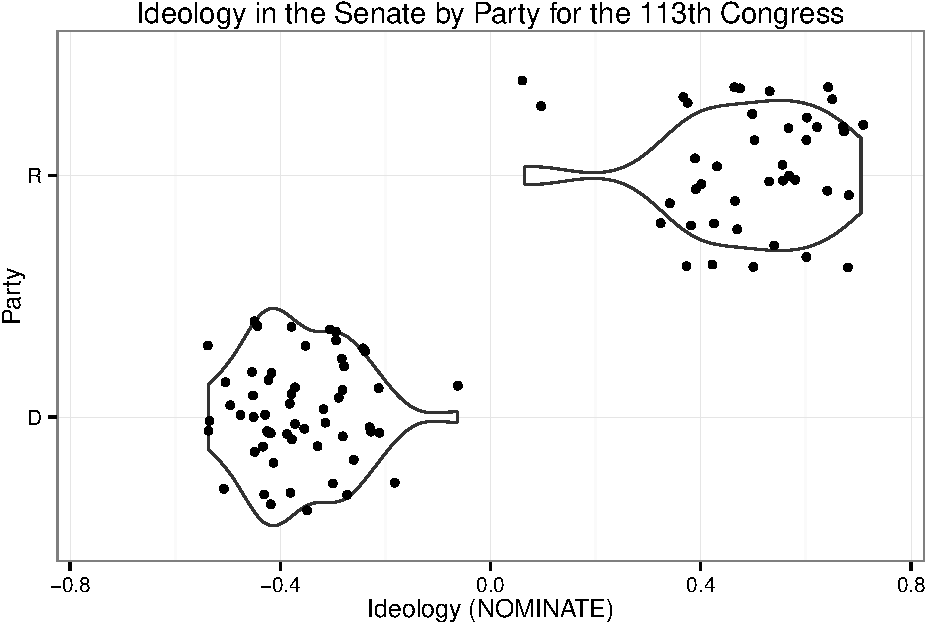
\includegraphics{trautlein_thesis_files/figure-latex/violin_113_senate-1} \end{center}
  
  \begin{center}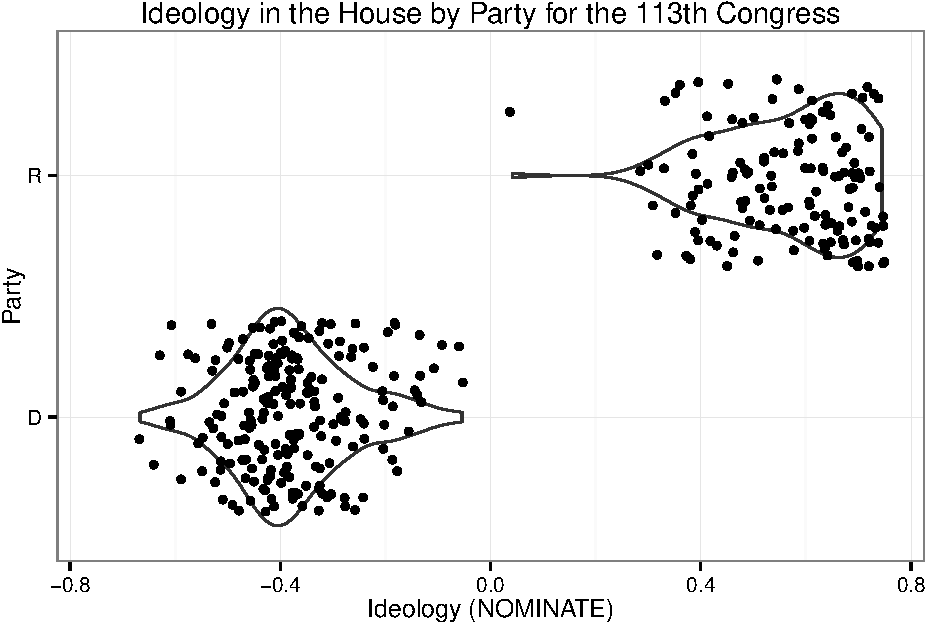
\includegraphics{trautlein_thesis_files/figure-latex/violin_113_house-1} \end{center}
  
  \begin{verbatim}
  Warning: Removed 103 rows containing non-finite values (stat_ydensity).
  \end{verbatim}
  
  \begin{verbatim}
  Warning: Removed 103 rows containing missing values (geom_point).
  \end{verbatim}
  
  \begin{center}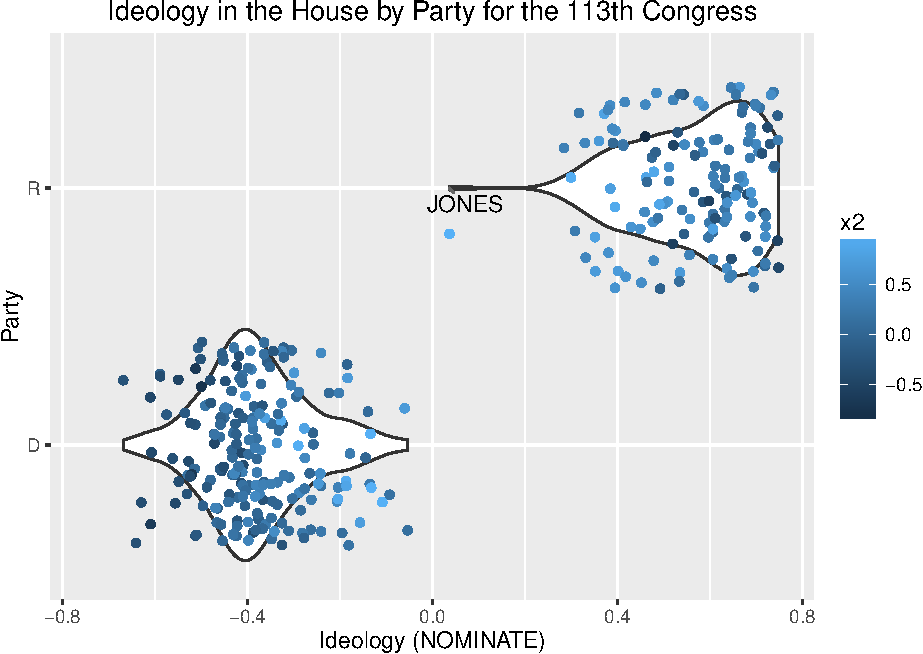
\includegraphics{trautlein_thesis_files/figure-latex/unnamed-chunk-1-1} \end{center}
  
  \begin{center}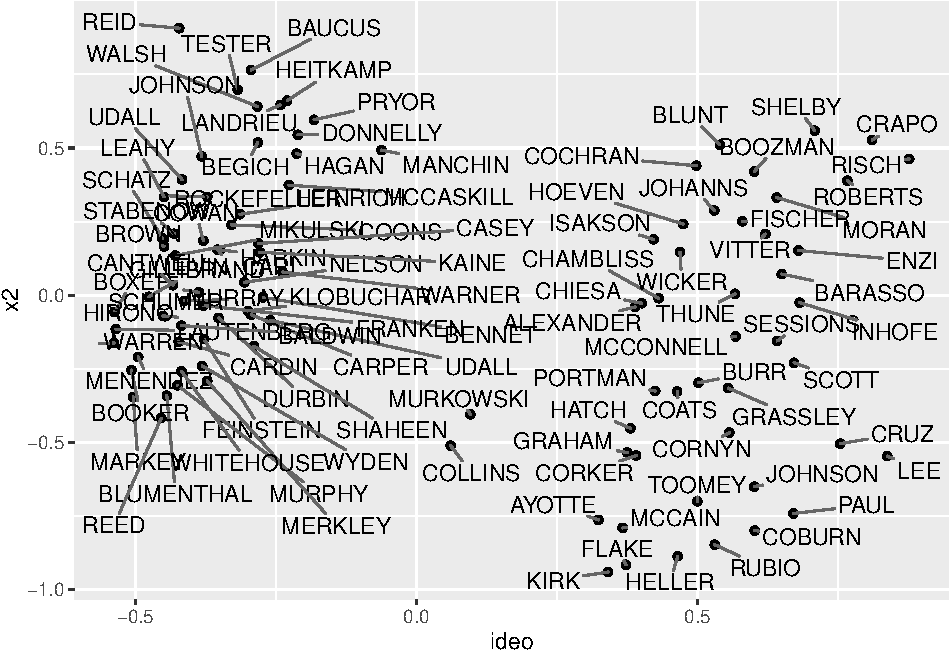
\includegraphics{trautlein_thesis_files/figure-latex/unnamed-chunk-1-2} \end{center}
  
  \begin{verbatim}
  Scale for 'colour' is already present. Adding another scale for
  'colour', which will replace the existing scale.
  \end{verbatim}
  
  \begin{center}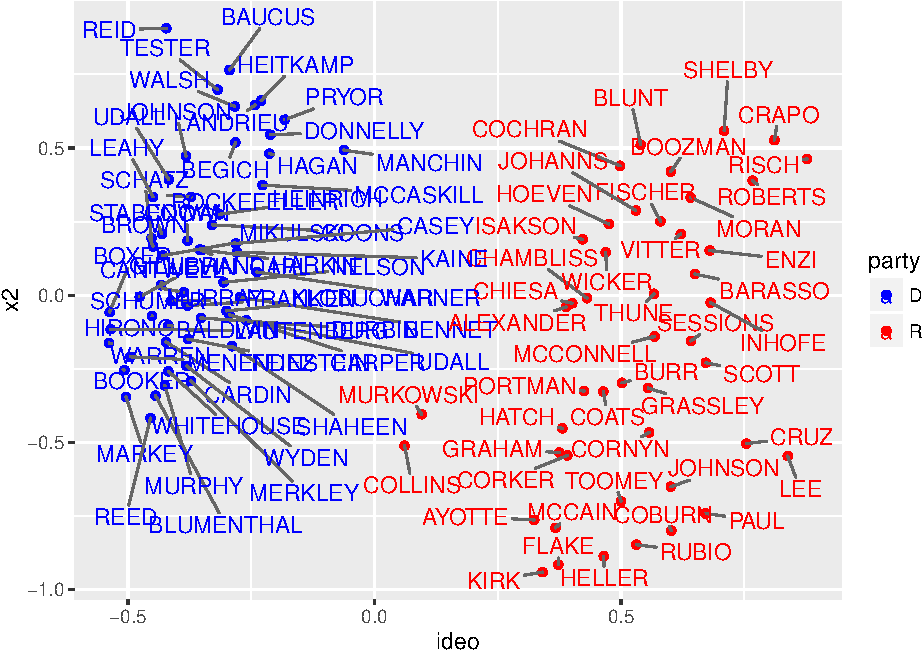
\includegraphics{trautlein_thesis_files/figure-latex/unnamed-chunk-1-3} \end{center}
  
  \begin{figure}[h!tbp]
  \centering
  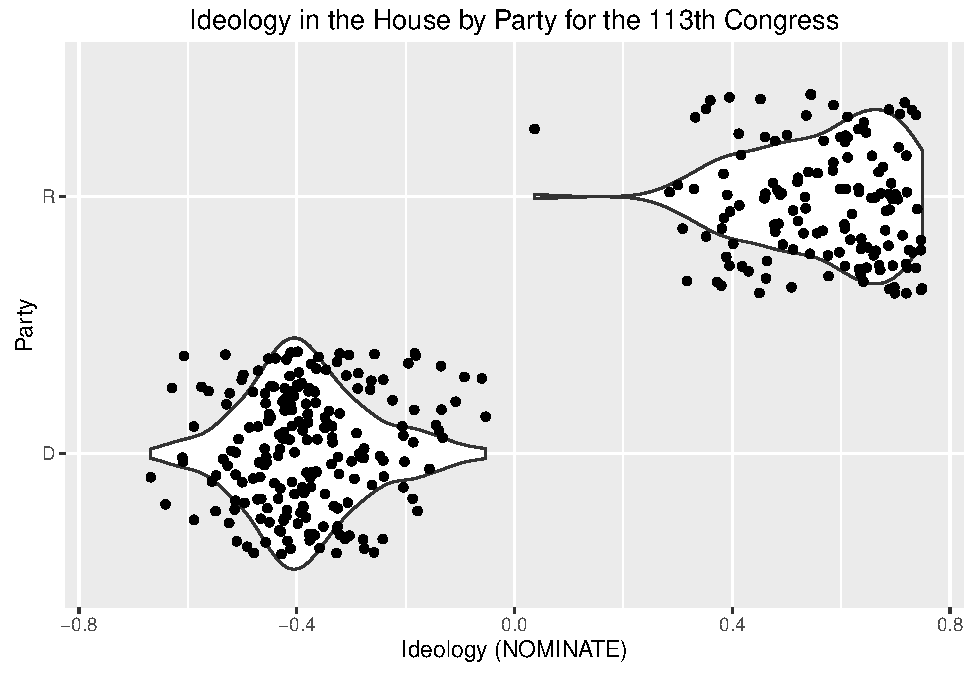
\includegraphics[angle = 0,scale = 1]{/Users/cus/thesis/trautlein_thesis/figures/PlotHouseMeans.pdf}
  \caption[Here is a caption]{\normalsize{Here is a caption}}
  \label{fig:def}
  \end{figure}
  
  \chapter{Dataset and Methodology}\label{dataset-and-methodology}
  
  \section{Dataset}\label{dataset}
  
  The dataset that I am using a special version of the DW-NOMINATE dataset
  that was created by Timothy Nokken and Keith Poole for a 2004 study to
  research congressional party defection throughout the history of the
  United States. What it shares with the DW-NOMINATE dataset is a first
  and second dimasion coordinate for each legislator across the
  Congresses. But it differs in that
  
  In order to properly subset my data I completely removed all
  independents from the dataset. In a later study it might be more useful
  to instead mark independents as a member of the Republican or Democratic
  party if they decide to caucus with them, such as Senator Sanders, an
  independent who caucuses with the Democrats, or Senator Joe Lieberman,
  and independent who also caucused with the Democrats. This did not seem
  to be a huge reduction in the total dataset size, as during the period
  this study looks at there were only sixteen total third party members of
  the Senate and only thirty-two total third party members in the
  House.\footnote{A significant percentage of these thirty-two are members of the Minnesota Farmer-Labor party or members of the Progressive party.}
  The variables a reader of this paper might be most interested in are:
  
  \begin{itemize}
  \itemsep1pt\parskip0pt\parsep0pt
  \item
    Congress Number, 1st Congress through 113th Congress
  \item
    ICPSR ID Number: A unique five digit code assigned to each legislator.
  \item
    State Code: A two digit code assigned by state.
  \item
    State Name: The name of the state the legislator is from.
  \item
    Party Code: 100 if a Democrat, 200 if a Republican, and many others
    exist for third parties.
  \item
    Name: The legislator's last name and occasionally first name and
    middle name initials.
  \item
    1st Dimension Coordinate: The most important dimension, can place a
    legislator in a party with over 80\% accuracy across most Congresses,
    and with 100\% accuracy in the current polarized environment.
  \item
    2nd Dimension Coordinate: The second dimension of voting data pulled
    out from the roll call votes. Across history it has often reflected
    disagreement within the parties. For example, in the 1960s within the
    Democratic and Republican party it reflected views on Civil Rights.
    Currently the dimension is not very predictive, but does help
    designate who is a member of the ``establishment'' versus the
    anti-establishment Members of Congress.
  \end{itemize}
  
  New variables were added during the cleaning and coding of the data.
  They are:
  
  \begin{itemize}
  \itemsep1pt\parskip0pt\parsep0pt
  \item
    Role: Blank if none, ``W'' if whip, ``L'' if leader, and ``S'' if
    Speaker.
  \item
    Leadership Position: ``Y'' if Role is not blank, ``N'' if Role is
    blank.
  \item
    Party Mean: The mean 1st dimension score of the party for the current
    Congress. Continuous and Numerical.
  \item
    Past Party Mean: The mean 1st dimension score of the party for the
    past Congress. Continuous and Numerical.
  \item
    Past Ideology: The 1st Dimension score for the Member of Congress for
    the past Congress.
  \end{itemize}
  
  \begin{longtable}[c]{@{}rrr@{}}
  \caption{Senate Mean Ideology By Party, 104th to 113th
  Congress}\tabularnewline
  \toprule
  Congress & Dem. Ideology & Rep.~Ideology\tabularnewline
  \midrule
  \endfirsthead
  \toprule
  Congress & Dem. Ideology & Rep.~Ideology\tabularnewline
  \midrule
  \endhead
  104 & -0.32581 & 0.35945\tabularnewline
  105 & -0.34491 & 0.39311\tabularnewline
  106 & -0.34037 & 0.38618\tabularnewline
  107 & -0.34046 & 0.39400\tabularnewline
  108 & -0.33088 & 0.36725\tabularnewline
  109 & -0.34327 & 0.41862\tabularnewline
  110 & -0.34360 & 0.44063\tabularnewline
  111 & -0.34595 & 0.44511\tabularnewline
  112 & -0.33365 & 0.50675\tabularnewline
  113 & -0.36271 & 0.53037\tabularnewline
  \bottomrule
  \end{longtable}
  
  \begin{longtable}[c]{@{}rrr@{}}
  \caption{House Mean Ideology By Party, 104th to 113th
  Congress}\tabularnewline
  \toprule
  Congress & Dem. Ideology & Rep.~Ideology\tabularnewline
  \midrule
  \endfirsthead
  \toprule
  Congress & Dem. Ideology & Rep.~Ideology\tabularnewline
  \midrule
  \endhead
  104 & -0.34211 & 0.48100\tabularnewline
  105 & -0.35750 & 0.51788\tabularnewline
  106 & -0.36091 & 0.54278\tabularnewline
  107 & -0.35842 & 0.55918\tabularnewline
  108 & -0.35822 & 0.58535\tabularnewline
  109 & -0.37146 & 0.60593\tabularnewline
  110 & -0.35234 & 0.64415\tabularnewline
  111 & -0.33722 & 0.67488\tabularnewline
  112 & -0.38793 & 0.68400\tabularnewline
  113 & -0.38112 & 0.69508\tabularnewline
  \bottomrule
  \end{longtable}
  
  \section{Methodology}\label{methodology}
  
  My goal is to understand how leadership positions affect the ideology of
  a Member of Congress. A Member of Congress during one Congress is my
  unit of observation. I looked at four independent variables and one
  dependent variable. The independent variables are:
  
  \begin{itemize}
  \itemsep1pt\parskip0pt\parsep0pt
  \item
    Past ideology: The 1st dimension score of the Member of Congress for
    the past Congress. Continuous and Numerical.
  \item
    Past party ideology: The mean 1st dimension score of the party for the
    past Congress. Continuous and Numerical.
  \item
    Current party ideology: The mean 1st dimension score of the party for
    the current Congress. Continuous and Numerical.
  \item
    Leadership status: If the Member of Congress is a ``leader,'' as
    described above in the dataset section. The variable of note. Binary.
  \end{itemize}
  
  I am looking to eventually use these variables to predict the response
  variable, current ideology. Current ideology is the 1st dimension score
  of the legislator of interest for the current Congress. I would expect
  the legislator's past ideology to be the most predictive, followed by
  the party's current ideology, with the third most predictive varible
  being the party's past ideology. Leadership status is expected to be the
  least predictive variable of the four tested for here.
  
  The few assumptions needed for a linear regression model had to be
  checked for. There is a chance that the model would be better
  represented by a non-linear model but due to the author's statistical
  knowhow a linear regression seemed most appropriate. Normality in the
  error terms as well as a constanct variance of the error terms also
  seemed to be met. The needed assumption that may have been hardest to
  work around was multicollinearity, or when predictor terms within the
  regression are able to predict each other with great accuracy. The
  variables around ideology could have some issues here and a future paper
  might try to further tease out whether there is a strong problem of
  colinearity in this dataset and model.
  
  \chapter{Results}\label{results}
  
  \section{Results for Complete
  Dataset}\label{results-for-complete-dataset}
  
  Some statistically significant results are found in my most basic
  regression. These are the linear regressions computed across all the
  available congressional sessions that have complete leader data in both
  the House and the Senate, from the 67th Congress (1921-1923) to the
  recent 113th Congress (2013-2015).
  
  \begin{table}[h]
  \centering
  \caption{Summary of Models Across All Years, House and Senate}
  \begin{tabular}{r|rrrr}
                         & Senate Ds & Senate Rs & House Ds & House Rs \\ \hline
  (Intercept)            & 0.00489   & 0.00259   & 0.01131  & 0.00405  \\
  cong\_ideo\_mean       & 0.51583   & 0.61344   & 0.73047  & 0.67749  \\
  last\_cong\_ideo\_mean & -0.38112  & -0.50989  & -0.57483 & -0.53415 \\
  last\_ideo             & 0.87467   & 0.87061   & 0.87636  & 0.85013  \\
  leaderY                & \textbf{-0.01863}  & 0.01289   & -\textbf{0.03022} & -0.00417 \\
  Adjusted R-Squared     & 0.802     & 0.781     & 0.781    & 0.824    \\
  N                      & 2239      & 1817      & 11380    & 9270    
  \end{tabular}
  \end{table}
  
  All of the control variables that were enlisted were found to be
  statistically signicant. These three variables were the idelogical mean
  of congress, the ideological mean of congress from the previous
  congressional session, and the congressperson's ideology from the
  previous congressional session. For all three of these variables across
  both parties in both the House and Senate the p-value was always less
  than 0.0001. It is clear that a legislator's current ideology would be
  affected by what their ideology was in the previous congressional
  session. While not as obvious, it also makes sense that you would need
  to understand the greater political environment that their party is in
  within their chamber. For example, if congresspeople as a whole were
  becoming more polarized at a rapid rate, as they are currently, you
  would expect a singular congressperson to be rapidly polarizing as well.
  Knowing how the party has changed from the previous Congress to the most
  recent one allows you to help control for this effect.
  
  \subsection{Democrats}\label{democrats}
  
  Across all of the years the leadership variable was statistically
  significant for the Senate Democrats and the House Democrats,
  represented by the bold text in Table 3.1 above. The Senate Democrats
  noticed a small shift, approximately a 0.02 leftward shift on the
  NOMINATE scale, indicating that leaders become slightly more liberal
  across Congresses than their non-leader counterparts. The result was not
  significant at a confidence level of the normal 0.05, but with a p-value
  of 0.059 it would be recognized as significant at a slighty higher
  confidence level. For reasons laid out farther below, I do not think
  that this is reason enough to disregard this result, as I would guess
  that this is an underestimate rather than an overestimate. The overall
  shift is small, only a 0.02 movement towards the more liberal side, but
  not insignificant.
  
  A statistically significant shift was also noticed among the House
  Democrats. They had an even more statistically significant result, with
  a p-value of about 0.015, a much stronger result than that found above
  with the Senate Democrats. It is strong enough that with the somewhat
  arbritrary confidence level of 0.05 the predictor remains signficant.
  The coefficient attached is also larger, 0.03, again with a leftwards
  shift farther towards the Democratic party extreme, farther towards
  congresspeople like Senator Sanders and Senator Brown and away from
  conservatives like Senator Collins and Senator Risch. Again, the overall
  shift is small but not worth disregarding, however if one was looking to
  predict the ideological score of a House Democrat you would not pick
  leadership status as one of your first predictors.
  
  \subsection{Republicans}\label{republicans}
  
  It is important to talk about the null results received for Republicans
  in both the House and Senate. While neither of the results were
  significant, the regression for the Senate did hint at a possible
  ideological change due to leadership, with a coefficient of 0.013
  towards the more conservative side. Accompanied by a p-value of 0.19
  they must be looked at skeptically, and instead perhaps taken as a hint
  for future study as opposed to a specific result. The coefficient found
  here is similar to the results found for the Democrats, they they moved
  more towards their party's extreme edges when they were leaders. It was
  not as strong as the coefficient found for either the House Democrats or
  the Senate Democrats, but it is no as weak as the Republican House,
  covered below. While significant was not found in this elementary
  regression, perhaps a regression with better controls and a stronger
  method might be able to find results that are not just statistically
  significant but also are statistically sound.
  
  The House Republicans however seem to be very far away from any possible
  impact of leadership on ideology. They had a p-value of 0.65, far away
  from any reasonable confidence level. Even if it had been significant
  the coefficient attached was incredibly small, 0.004, towards the more
  moderate wing fo the Republican party or the Democratic party itself.
  These results are not in sync with the results found for the other three
  groups analyzed here, and I might suggest that looking at
  
  \subsection{Comments on Null Results}\label{comments-on-null-results}
  
  With the model I have created I think it is likely that the significance
  of leadership on ideology is underestimated. The change in leadership
  could have an effect on how the ideology of an entire caucus moves.
  Speaker Ryan right now is trying hard to make his ideology the ideology
  of the entire party, as he has pushed his agenda of ``Confident
  America'' (Steinhauer 2016). Ryan is closer to the mean ideological
  scores of the Freedom Caucus, and one would imagine that a concerted
  effort to continue to elect leaders of more extreme ideologies might
  allow the rest of the party to move along with them towards their more
  extreme wings (Enten 2015).
  
  Also the model might underestimate the importance of being a leader for
  a few another reasons. For example, leaders are a part of the data on
  the last congressional ideological mean and the current congressional
  ideological mean. Also leaders might have altered their early,
  pre-leader ideology because they expected or wanted to become leaders in
  the future. All of these could account for the differences among the
  significance of the leadership variable among the Democrats when
  compared to the Republicans. Perhaps Republicans were more likely to
  know they wanted to pursue leadership since they first entered office,
  or maybe they were more likely to shift along with their leaders,
  causing the entire mean of the party to move, possibly nullifing the
  effects of a leader's move.
  
  \section{Results for Subsets of
  Dataset}\label{results-for-subsets-of-dataset}
  
  I took subsets of the data by Congressional periods to try to see if
  leaders were ever more important across certain time periods then they
  were over the entire dataset. There are many different ways to break up
  Congress, one way suggested by (Stewart 2012, 96--97) is the breaking
  into six different eras, or systems, of which only three are during the
  time period that was able to be coded wih
  leaders.\footnote{The rest were pre-1921 and before my data was able to be clearly coded due how Congressional leadership existed back then.}
  They are:
  
  \begin{itemize}
  \itemsep1pt\parskip0pt\parsep0pt
  \item
    \textbf{Industrial System}: 1921-1932: Actually 1894-1932, but for the
    purposes of our coding only a smaller amount of it can be analyzed. A
    party of industry and a party of labor, with northern and southern
    regionalism factoring into parties heavily. Republicans were primarily
    northern and industrial, whereas Democrats were primarily southern and
    labor focused.
  \item
    \textbf{New Deal System}: 1932-1972: Democrats become more liberal as
    the Republicans become more conservative compared to industrial
    system, but the regionalism does not completely fade away.
  \item
    \textbf{Candidate-centered system}: 1972-present: After the tension
    that existed in the United States in the sixties, the regional
    importance shifts away as ideology begins to matter more and
    polarization of the parties continues (Stewart 2012, 96).
  \end{itemize}
  
  This system of breaking up the parties is not the only manner in which
  one could break them up, and subscribes to the views that are not taken
  as true across all of the political science literature. Some push both
  the Industrial and New Deal system together as one Congressional period.
  Yet the years themselves above seem to delineate good beginning breaking
  points for me to subset the data.
  
  \subsection{Republicans}\label{republicans-1}
  
  Subsets were not useful to explain how House Republicans voted. During
  all of the systems the p-value were relatively high. That being said the
  subsetting did reduce the p-value by a significant amount, bringing the
  p-value for all three eras to between 0.22 and 0.26. This is an
  improvement when compared to the original 0.65 value received, but not
  enought to pass a positive judgement on the effects of these values. The
  coefficients were also stronger than they were when all of the systems
  were lumped together, but they still are smaller than the absolute value
  of the coefficients that exist for the Republicans in the House and
  Senate.
  
  The values obtained for the Senate Republicans did not all become more
  explanatory as they did for the House Republicans. The p-value increases
  for all eras except for the New Deal era, when it moves down to 0.14.
  But during the Industrial and Candidate-centered systems the p-values
  increase dramatically to point where they seem unable to be rationalized
  in any way. So again subsetting is overall mostly ineffective at helping
  try to tease out statistically significant ideological change due to a
  leadership position.
  
  \subsection{Democrats}\label{democrats-1}
  
  Subsetting is more effective in talking about the importance of
  leadership when it comes to ideological change among House Democrats
  however. Null results are found for both the industrial and candidate
  centered systems, with p-values reaching far above 0.20. However for the
  House Democrats during the New Deal era, from 1932-1972 or the 73rd
  Congress to the 92nd Congress, the subsetting increases the significance
  of the data. Not only does the p-value decrease from the all full
  dataset p-value of 0.015 to the even stronger p-value of 0.006 but the
  coefficient increases as well, doubling from a 0.03 shift towards the
  left to a 0.06 shift towards the left. This is a very significant shift
  among the NOMINATE scale, so this will be revisted in the discussion of
  the results later. It did not come at a reduction of the importance of
  the other variables, which stayed statistically and substantively
  significant.
  
  Subsetting is also effective in explaining during which congressional
  systems leadership has its greatest effect on the ideology of Senate
  Democrats. Again, the period in which the strongest p-value and
  coefficient is found is during the New Deal system (1932-1973). The
  p-value for this time period is 0.08 and its corresponding coefficient
  is a 0.03 shift towards the left, stronger by 0.01 than the baseline
  analysis of the Senate Democrats. Due to slowed polarization in the
  Senate compared to the House this ideological shift means more than it
  would otherwise.
  
  \section{Conclusion}\label{conclusion}
  
  Overall it is clear that Democrats were more likely to have significant
  results than Republicans. The New Deal system was also more likely to
  produce significant results than the other systems were. In the
  discussion section below I expound on these results and try to tie them
  into my earlier hypotheses about how leadership positions affect
  ideology.
  
  \chapter{Discussion and Conclusion}\label{discussion-and-conclusion}
  
  \section{Discussion}\label{discussion}
  
  As discusssed above, there were five different possible hypotheses that
  we were able to come up with - one null hypothesis and four alternative
  hypotheses. Again, I will repeat all five of them below.
  
  \begin{enumerate}
  \def\labelenumi{\arabic{enumi}.}
  \itemsep1pt\parskip0pt\parsep0pt
  \item
    A null result is found - the leaders and non-leaders do not change in
    significantly different ways.
  \item
    Leaders move to be more conservative, or right-leaning, when compared
    to non-leaders.
  \item
    Leaders move to be more liberal, or left-leaning, when compared to
    non-leaders.
  \item
    Leaders move to be more moderate, or centrist, when compared to
    non-leaders.
  \item
    Leaders move to be more extreme when compared to non-leaders.
  \end{enumerate}
  
  Luckily I need not pick only one hypothesis above to describe the
  phenomena observed because three of the hypotheses seemed to be correct,
  depending on the circumstance.
  
  Firstly, the null hypothesis seems to be correct in the vast majority of
  situations. While the
  
  Secondly, the Democrats seemed to be explained well by the third
  hypothesis above, that leaders become more liberal when compared to
  non-leaders. There are a number of reasons why this could take place.
  Perhaps one of the most largest reasons I see being the case is that one
  of the largest threats for these leaders is that they are receiving a
  large amount of media attention and may attract a primary opponent.
  
  \textless{}\textless{} ALSO GOING TO REFER TO EXTEMISM LITERATURE THAT I
  TALKED ABOUT IN LIT REVIEW, MAY EXPAND ON IT IN LIT REVIEW AS WELL
  \textgreater{}\textgreater{}
  
  Thirdly, the fifth hypothesis also can follow from the third hypothesis
  above because there are only results on the Democratic side.
  
  \section{Conclusion}\label{conclusion-1}
  
  This study was particularly important because while a reasonable amount
  of information exists about how leaders are chosen to their positions
  based on their ideology it was not completely clear about how their
  ideology might shift after they have been selected by their fellow
  members of Congress. This thesis has looked to narrow our gap of
  understanding of these topics. However, more research is need in the
  long run especially research that involves stronger statistical methods
  that can better compensate for the sometimes small number of
  observations that exist on the models that make reference to the
  leaders. Research could also be done on whether these leaders are
  encouraging partisanship in Congress due to their ideology or halting
  it, as one of the key pieces of information found within this dataset is
  the great partisanship and polarization of the two dominating parties
  within American politics.
  
  \backmatter
  
  \chapter{Bibliography}\label{bibliography}
  
  \noindent
  
  \setlength{\parindent}{-0.20in} \setlength{\leftskip}{0.20in}
  \setlength{\parskip}{8pt}
  
  Brewer, Mark D, and Jeffrey M Stonecash. 2015. \emph{Polarization and
  the Politics of Personal Responsibility}. Oxford University Press.
  
  Clausen, Aage R, and Clyde Wilcox. 1987. ``Policy Partisanship in
  Legislative Leadership Recruitment and Behavior.'' \emph{Legislative
  Studies Quarterly}. JSTOR, 243--63.
  
  Cox, Gary W, and Mathew D McCubbins. 2005. \emph{Setting the Agenda:
  Responsible Party Government in the US House of Representatives}.
  Cambridge University Press.
  
  Dodd, Lawrence C, and Bruce I Oppenheimer. 2012. \emph{Congress
  Reconsidered}. SAGE.
  
  Enten, Harry. 2015. ``What Paul Ryan Has That Kevin McCarthy and John
  Boehner Don't.'' \emph{FiveThirtyEight}.
  
  Evans, C Lawrence, and Walter J Oleszek. 1999. ``The Strategic Context
  of Congressional Party Leadership.'' In \emph{Congress \&Amp; the
  Presidency: A Journal of Capital Studies}, 26:1--20. 1. Taylor \&amp;
  Francis.
  
  Grofman, Bernard, William Koetzle, and Anthony J McGann. 2002.
  ``Congressional Leadership 1965--96: A New Look at the Extremism Versus
  Centrality Debate.'' \emph{Legislative Studies Quarterly} 27 (1). Wiley
  Online Library: 87--105.
  
  Harris, Douglas B, and Garrison Nelson. 2008. ``Middlemen No More?
  Emergent Patterns in Congressional Leadership Selection.'' \emph{PS:
  Political Science \&Amp; Politics} 41 (01). Cambridge Univ Press:
  49--55.
  
  Heberlig, Eric, Marc Hetherington, and Bruce Larson. 2006. ``The Price
  of Leadership: Campaign Money and the Polarization of Congressional
  Parties.'' \emph{Journal of Politics} 68 (4). Wiley Online Library:
  992--1005.
  
  Holcombe, Randall G. 2006. \emph{Public Sector Economics: The Role of
  Government in the American Economy}. Prentice Hall.
  
  Jessee, Stephen, and Neil Malhotra. 2010. ``Are Congressional Leaders
  Middlepersons or Extremists? Yes.'' \emph{Legislative Studies Quarterly}
  35 (3). Wiley Online Library: 361--92.
  
  MacDonald, Stuart Elaine, and George Rabinowitz. 1987. ``The Dynamics of
  Structural Realignment.'' \emph{American Political Science Review} 81
  (03). Cambridge Univ Press: 775--96.
  
  May, John D. 1973. ``Opinion Structure of Political Parties: The Special
  Law of Curvilinear Disparity.'' \emph{Political Studies} 21 (2). Wiley
  Online Library: 135--51.
  
  Mayhew, David R. 2004. \emph{Congress: The Electoral Connection}. 2nd
  Edition. Yale University Press.
  
  Nokken, Timothy P, and Keith T Poole. 2004. ``Congressional Party
  Defection in American History.'' \emph{Legislative Studies Quarterly} 29
  (4). Wiley Online Library: 545--68.
  
  Poole, Keith T, and Howard Rosenthal. 1991. ``Patterns of Congressional
  Voting.'' \emph{American Journal of Political Science}. JSTOR, 228--78.
  
  Poole, Keith T, and Howard L Rosenthal. 2007. \emph{Ideology and
  Congress}. Transaction Publishers.
  
  Rohde, David W. 1991. ``Parties and Leaders in the Postreform
  Congress.'' \emph{Chicago, IL: Uni}.
  
  Sinclair, Barbara, Roger H Davidson, Walter J Oleszek, Charles O Jones,
  Thomas E Mann, Norman J Ornstein, James L Sundquist, Frank H Mackaman,
  Joseph Cooper, and G Calvin Mackenzie. 1983. ``Purposive Behavior in the
  US Congress: A Review Essay.'' JSTOR.
  
  Steinhauer, Jennifer. 2016. ``Paul Ryan, a Mirage Candidate, Wages a
  Parallel Campaign.'' \emph{The New York Times}.
  
  Stewart, Charles Haines. 2012. \emph{Analyzing Congress: The New
  Institutionalism in American Politics}. 2nd ed. Norton.
  
  Theriault, Sean M. 2008. \emph{Party Polarization in Congress}.
  Cambridge University Press.


  % Index?

\end{document}

